\documentclass[11pt,english]{beamer}

\usepackage[T1]{fontenc}
\usepackage[utf8]{inputenc}
\usepackage[french, english]{babel}
\usepackage{hyperref}
\usepackage{tikz}
\usetikzlibrary{shapes,snakes}
\usepackage{ulem}
\usepackage{xcolor, colortbl}
\usepackage{mathtools}
\usepackage{xcolor}
\usepackage{rotating}
\usepackage{lipsum}

\usepackage{varwidth}

\usepackage[style=alphabetic]{biblatex}
\beamertemplatenavigationsymbolsempty

\bibliography{Biblio.bib}

\usetikzlibrary{arrows}
\usetikzlibrary{positioning}

\definecolor{mygreen}{rgb}{0.55, 0.71, 0.0}


\newcommand\blfootnote[1]{%
 \begingroup
  \renewcommand\thefootnote{}\footnote{#1}%
  \addtocounter{footnote}{-1}%
  \endgroup
}

\institute[ENS Rennes] % (optional, but mostly needed)
{


  \begin{columns}
    \column{0.45\linewidth}
    \center
    
\includegraphics[scale=0.15]{ENS}\\
    Computer science department\\
    ENS Rennes

    \column{0.45\linewidth}
    \center
    
\includegraphics[scale=0.25]{Linkmedia}

    Linkmedia project\\
    IRISA
  \end{columns}

}

\usetheme{AnnArbor}
\usecolortheme{beaver}

\title{DeepVoice}
\subtitle{Extracting meaningful signal representation for Speaker Recognition
\\  using deep architectures}

\author[Hutin,Sun,Truffet]{Rémi Hutin, Rémy Sun, Raphaël Truffet \\ Supervisors : Guillaume Gravier and Vedran Vukoti\'c}


\date{May 9, 2017}


\AtBeginSection[]{
    \begin{frame}
        \frametitle{Outline}
        \tableofcontents[currentsection,hideothersubsections]
    \end{frame}
}

\setbeamertemplate{navigation symbols}{}%remove navigation symbols


\begin{document}

\begin{frame}
    \titlepage
\end{frame}

\begin{frame}
	\begin{figure}
		\centering
       	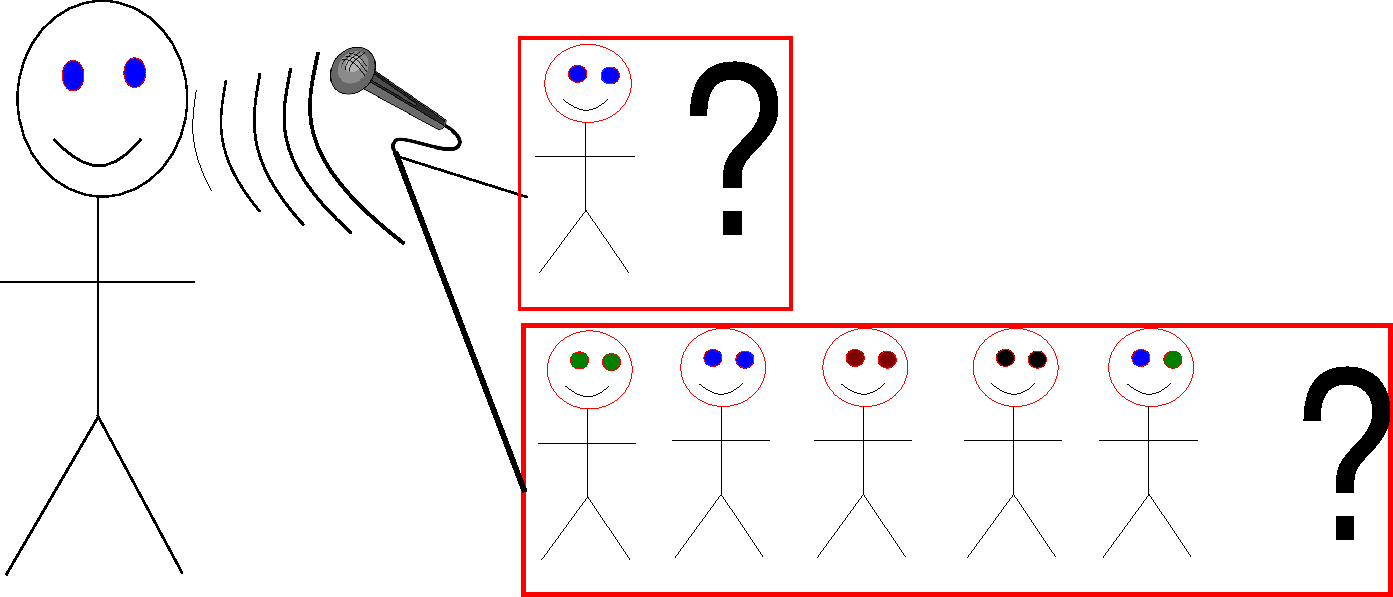
\includegraphics[scale = 0.5]{intro.pdf}
	\end{figure}
\end{frame}


\begin{frame}
	\begin{figure}
		\centering
        \begin{tikzpicture}[box/.style={draw,rounded corners,align=center},
                            bubble/.style={draw,circle,align=center},
                            vec/.style={draw,rectangle,align=center, text width=0.1cm, text height=0.1cm},
                            barre/.style={draw,cross out,align=center}
                           ]
        \visible<2-3>
        {
        \node[bubble] (eq) {= ?};
        }
        \node[box,fill=blue!16, left =1cm of eq] (1) {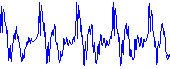
\includegraphics[scale = 0.5]{signal.png}};
        \node[box,fill=green!16, right =1cm of eq] (2) {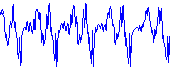
\includegraphics[scale = 0.5]{signal180.png}};


        \visible<2-3>
        {
        \draw[->] (1) -- (eq);
        \draw[->] (2) -- (eq);
        }

        \visible<3>
        {
        \node[barre, color=red, thick, text width = 1cm, text height = 1cm] {};
        }

        \visible<4->
        {
        \node[box,fill=black!70, below =1cm of 1] (bb1) {
\includegraphics[scale = 0.2]{options_icon.pdf}};
        \node[box,fill=black!70, below =1cm of 2] (bb2) {
\includegraphics[scale = 0.2]{options_icon.pdf}};
        \draw[->] (1) -- (bb1);
        \draw[->] (2) -- (bb2);
        }

        \visible<5->
        {
            \node[vec,fill=blue!16, below =1cm of bb1] (v11) {};
            \node[vec,fill=blue!16, below =0cm of v11] (v12) {};
            \node[vec,fill=blue!16, below =0cm of v12] (v13) {};
            \node[vec,fill=blue!16, below =0cm of v13] (v14) {};
            \node[vec,fill=blue!16, below =0cm of v14] (v15) {};

            \node[vec,fill=green!16, below =1cm of bb2] (v21) {};
            \node[vec,fill=green!16, below =0cm of v21] (v22) {};
            \node[vec,fill=green!16, below =0cm of v22] (v23) {};
            \node[vec,fill=green!16, below =0cm of v23] (v24) {};
            \node[vec,fill=green!16, below =0cm of v24] (v25) {};

            \draw[->] (bb1) -- (v11);
            \draw[->] (bb2) -- (v21);
        }


        \visible<6->
        {
            \node[bubble, fill=green!40, thick, below =3.5cm of eq] (eq2) {= ?};

            \draw[->] (v13) -- (eq2);
            \draw[->] (v23) -- (eq2);
        }
        \end{tikzpicture}
        \end{figure}
\end{frame}


\begin{frame}
    \begin{figure}
            \centering
    \begin{tikzpicture}[box/.style={draw,rounded corners,align=center},
                        vec/.style={draw,rectangle,align=center, text width=0.1cm, text height=0.1cm},
                        bb2/.style={draw,rectangle,align=center, text width=0.35cm, text height=0.35cm}]

        \node[box,fill=blue!16] (s) {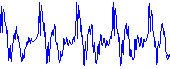
\includegraphics[scale = 0.6]{signal.png}};
        \node[box,fill=black!70, right =2cm of s] (bb) {
\includegraphics[scale = 0.4]{options_icon.pdf}};
        \node[vec,fill=blue!16, right =2cm of bb] (v3) {};
        \node[vec,fill=blue!16, below =0cm of v3] (v4) {};
        \node[vec,fill=blue!16, below =0cm of v4] (v5) {};
        \node[vec,fill=blue!16, above =0cm of v3] (v2) {};
        \node[vec,fill=blue!16, above =0cm of v2] (v1) {};

        \draw[->] (s) -- (bb);
        \draw[->] (bb) -- (v3);


        \visible<2->
        {
        \node[below right=-1.3cm of bb] (puzzle) {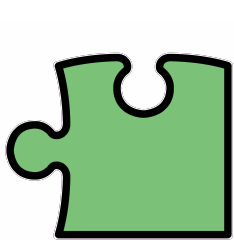
\includegraphics[scale = 0.1]{puzzle.png}};
        \node[below =1cm of puzzle] (dnn) {Deep Neural Networks};
        \draw[->] (dnn) -- (puzzle);
        }
    \end{tikzpicture}
    \end{figure}
\end{frame}


\begin{frame}
    \frametitle{Outline}
    \tableofcontents[hideallsubsections]
\end{frame}


\section{Signal representation for speaker recognition}

\begin{frame}
  \frametitle{Signal processing workflow}
    \centering
    \begin{tikzpicture}[box/.style={draw,rounded corners,align=center},barre/.style={draw,cross out,align=center}]
    \node[box,fill=blue!16] (a) {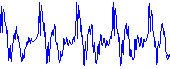
\includegraphics[scale=0.25]{signal.png}\\Signal};
    \node[box,fill=green!16,right =0.6cm of a] (f2) {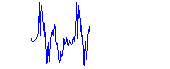
\includegraphics[scale=0.25]{fen2.png}};
    \node[box,fill=green!16,above =0.6cm of f2] (f1) {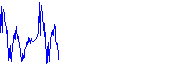
\includegraphics[scale=0.25]{fen1.png}};
    \node[below =0.8cm of f2] (f3) {\dots};
    \node[box,fill=green!16,below =0.6cm of f3] (fn) {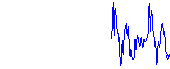
\includegraphics[scale=0.25]{fenn.png}};
    \draw[->] (a) -- (f1);
    \draw[->] (a) -- (f2);
    \draw[->] (a) -- (fn);



    \node[box,fill=orange!16, right = 0.6cm of f1] (c1) {cepstral\\coefficients};
    \node[box,fill=orange!16, right = 0.6cm of f2] (c2) {cepstral\\coefficients};
    \node[right = 2cm of f3] (c3) {\dots};
    \node[box,fill=orange!16, right = 0.6cm of fn] (cn) {cepstral\\coefficients};

    \draw[->] (f1) -- (c1);
    \draw[->] (f2) -- (c2);
    \draw[->] (fn) -- (cn);


    \node[box,fill=cyan!16, right = 0.6cm of c2] (sv) {Supervector};
    \node[box,fill=red!16, above = 1.5cm of sv] (ubm) {UBM};

    \draw[->] (c1) -- (sv);
    \draw[->] (c2) -- (sv);
    \draw[->] (cn) -- (sv);
    \draw[->] (ubm) -- (sv);

    \node[box,fill=yellow!16, right = 0.6cm of sv] (iv) {I-vectors};
    \draw[->] (sv) -- (iv);
    \end{tikzpicture}
\end{frame}


\begin{frame}
  \frametitle{Question}

	\centering
	{\Huge Can we do better than i-vectors? \par}

\end{frame}


\begin{frame}
  \frametitle{Signal processing workflow}
    \centering
    \begin{tikzpicture}[box/.style={draw,rounded corners,align=center},barre/.style={draw,cross out,align=center}]
    \node[box,fill=blue!16] (a) {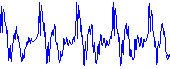
\includegraphics[scale=0.25]{signal.png}\\Signal};
    \node[box,fill=green!16,right =0.6cm of a] (f2) {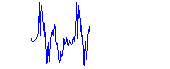
\includegraphics[scale=0.25]{fen2.png}};
    \node[box,fill=green!16,above =0.6cm of f2] (f1) {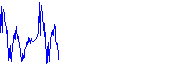
\includegraphics[scale=0.25]{fen1.png}};
    \node[below =0.8cm of f2] (f3) {\dots};
    \node[box,fill=green!16,below =0.6cm of f3] (fn) {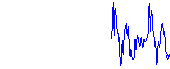
\includegraphics[scale=0.25]{fenn.png}};
    \draw[->] (a) -- (f1);
    \draw[->] (a) -- (f2);
    \draw[->] (a) -- (fn);



    \node[box,fill=orange!16, right = 0.6cm of f1] (c1) {cepstral\\coefficients};
    \node[box,fill=orange!16, right = 0.6cm of f2] (c2) {cepstral\\coefficients};
    \node[right = 2cm of f3] (c3) {\dots};
    \node[box,fill=orange!16, right = 0.6cm of fn] (cn) {cepstral\\coefficients};

    \draw[->] (f1) -- (c1);
    \draw[->] (f2) -- (c2);
    \draw[->] (fn) -- (cn);


    \node[box,fill=cyan!16, right = 0.6cm of c2] (sv) {Supervector};
    \node[box,fill=red!16, above = 1.5cm of sv] (ubm) {UBM};

    \draw[->] (c1) -- (sv);
    \draw[->] (c2) -- (sv);
    \draw[->] (cn) -- (sv);
    \draw[->] (ubm) -- (sv);

    \node[barre, right = 0.6cm of sv] (iv) {I-vectors};
    \node[box,fill=yellow!16, below = 1cm of iv] (ow) {\Large Our work};
    \draw[->] (sv) -- (iv);
    \draw[->] (sv) -- (ow);
    \end{tikzpicture}
\end{frame}


\section{Deep learning}

\begin{frame}
  \frametitle{Use of Deep Neural Networks (DNN)}

Deep neural networks are interesting because:
\begin{itemize}
\item \textbf{Non-linear} feature extraction
\item<2-> They naturally generate several level of representation
\item<3-> They bring out unsuspected features
\item<4-> There is a multitude of architectures


\end{itemize}

\end{frame}

\begin{frame}
  \frametitle{Formal neuron}
\def\layersep{2.5cm}


\begin{figure}
\centering
\begin{tikzpicture}[shorten >=1pt,->,draw=black!50, node distance=\layersep]
    \tikzstyle{every pin edge}=[<-,shorten <=1pt]
    \tikzstyle{neuron}=[ellipse,fill=black!25,minimum size=17pt,inner sep=0pt]
    \tikzstyle{input neuron}=[neuron, fill=green!50];
    \tikzstyle{output neuron}=[neuron, fill=red!50];
    \tikzstyle{hidden neuron}=[neuron, fill=blue!50];
    \tikzstyle{hidden neuron back}=[neuron, fill=orange!50];
    \tikzstyle{annot} = [text width=8em, text centered]

    % Draw the input layer nodes
    \foreach \name / \y in {1,...,4}
    % This is the same as writing \foreach \name / \y in {1/1,2/2,3/3,4/4}
        \node[input neuron, pin=left:] (I-\name) at (0,-\y) {$a_\y$};

    % Draw the hidden layer nodes
    \foreach \name / \y in {1,...,1}
        {
        \visible<-2>{\path[yshift=-1.5cm]
            node[hidden neuron] (H-\name) at (\layersep,-\y cm) {};}
        \visible<3->{\path[yshift=-1.5cm]
            node[hidden neuron back] (H-\name) at (\layersep,-\y cm) {};}
        }

    % Draw the output layer node
    \node[output neuron, right of=H-1] (O) {$e = f(WA + b)$};

    % Connect every node in the input layer with every node in the
    % hidden layer.
    \foreach \source in {1,...,4}
        \foreach \dest in {1,...,1}
            \path (I-\source) edge (H-\dest);

    % Connect every node in the hidden layer with the output layer
    \foreach \source in {1,...,1}
        \path (H-\source) edge (O);

    % Annotate the layers
    \node[annot,below of=H-1, node distance=1cm] (wb) {Weight $W\visible<3->{'}$\\Bias $b\visible<3->{'}$};
    \node[annot,above of=H-1, node distance=1cm] (n) {Neuron};
    \node[annot,above of=I-1, node distance=1cm] (ia) {Input A};

    \visible<2->{
    \node[annot,above =2cm of O, node distance=1cm] (md) {minimize : $\|e - e^* \|$};

    \path (O) edge (md);
    }
    \visible<3->{
    \path (md) edge (H-1);
    }
\end{tikzpicture}

\end{figure}

\blfootnote{LeCun, Y., Bottou, L., Bengio, Y., and Haffner, P. (1998d). Gradient-based learning applied to document recognition. Proceedings of the IEEE, 86(11), 2278–2324.}

\end{frame}

\begin{frame}
  \frametitle{Neural network}
\def\layersep{1.8cm}


\begin{figure}
\centering
\begin{tikzpicture}[shorten >=1pt,->,draw=black!50, node distance=\layersep]
    \tikzstyle{every pin edge}=[<-,shorten <=1pt]
    \tikzstyle{neuron}=[circle,fill=black!25,minimum size=17pt,inner sep=0pt]
    \tikzstyle{input neuron}=[neuron, fill=green!50];
    \tikzstyle{output neuron}=[neuron, fill=red!50];
    \tikzstyle{hidden neuron}=[neuron, fill=blue!50];
    \tikzstyle{hidden neuron back}=[neuron, fill=orange!50];
    \tikzstyle{annot} = [text width=4em, text centered]

    % Draw the input layer nodes
    \foreach \name / \y in {1,...,4}
    % This is the same as writing \foreach \name / \y in {1/1,2/2,3/3,4/4}
        \node[input neuron, pin=left:] (I-\name) at (0,-\y) {$a_\y$};

    % Draw the hidden layer nodes
    \foreach \name / \y in {1,...,5}
        {
        \visible<1>{\path[yshift=0.5cm]
            node[hidden neuron] (H1-\name) at (\layersep,-\y cm) {};}
        \visible<2>{\path[yshift=0.5cm]
            node[hidden neuron back] (H1-\name) at (\layersep,-\y cm) {};}
        }

    \foreach \name / \y in {1,...,4}
        {
        \visible<1>{\path
            node[hidden neuron] (H2-\name) at (2*\layersep,-\y cm) {};}
        \visible<2>{\path
            node[hidden neuron back] (H2-\name) at (2*\layersep,-\y cm) {};}
        }

    \foreach \name / \y in {1,...,5}
        {
        \visible<1>{\path[yshift=0.5cm]
            node[hidden neuron] (H3-\name) at (3*\layersep,-\y cm) {};}
        \visible<2->{\path[yshift=0.5cm]
            node[hidden neuron back] (H3-\name) at (3*\layersep,-\y cm) {};}
        }
    % Draw the output layer node
    \node[output neuron,pin={[pin edge={->}]right:Output}, right of=H3-3] (O) {};

    % Connect every node in the input layer with every node in the
    % hidden layer.

    \foreach \source in {1,...,4}
        \foreach \dest in {1,...,5}
            {\path (I-\source) edge (H1-\dest);}


    \foreach \source in {1,...,4}
        \foreach \dest in {1,...,5}
            \path (I-\source) edge (H1-\dest);

    \foreach \source in {1,...,5}
        \foreach \dest in {1,...,4}
            \path (H1-\source) edge (H2-\dest);

    \foreach \source in {1,...,4}
        \foreach \dest in {1,...,5}
            \path (H2-\source) edge (H3-\dest);

    \foreach \source in {1,...,5}
        \path (H3-\source) edge (O);


    % Annotate the layers
    \node[annot,above of=H1-1, node distance=1cm] (hl1) {Hidden layer 1};
    \node[annot,right of=hl1] (hl2) {Hidden layer 2};
    \node[annot,right of=hl2] (hl3) {Hidden layer 3};
    \node[annot,right of=hl3] {Output layer};
    \node[annot,left of=hl1] {Input layer};

    \node[annot,below of=H1-5, node distance=1cm] (wb1) {$W\visible<2>{'}_1$, $b\visible<2>{'}_1$};
    \node[annot,right of=wb1] (wb2) {$W\visible<2>{'}_2$, $b\visible<2>{'}_2$};
    \node[annot,right of=wb2] (wb3) {$W\visible<2>{'}_3$, $b\visible<2>{'}_3$};
\end{tikzpicture}

\end{figure}

\end{frame}

\begin{frame}
  \frametitle{Autoencoder}
\def\layersep{1.8cm}
    \begin{figure}
    \centering
\begin{tikzpicture}[yscale=0.7, shorten >=1pt,->,draw=black!50, node distance=\layersep]
    \tikzstyle{every pin edge}=[<-,shorten <=1pt]
    \tikzstyle{neuron}=[circle,fill=black!25,minimum size=17pt,inner sep=0pt]
    \tikzstyle{input neuron}=[neuron, fill=green!50];
    \tikzstyle{output neuron}=[neuron, fill=red!50];
    \tikzstyle{hidden neuron}=[neuron, fill=blue!50];
    \tikzstyle{hidden neuron back}=[neuron, fill=orange!50];
    \tikzstyle{annot} = [text width=10em, text centered]

    \visible<2>{
        \path [draw, thick, fill=yellow!20] (-1.2,0.5) rectangle (4.5,-5.6);
    }
    \visible<3->{
        \path [draw, thick] (-1.2,0.5) rectangle (4.5,-5.6);
    }
    \visible<3>{
        \path [draw, thick,  fill=yellow!20] (2.7,0.3) rectangle (8.4,-5.8);
    }
    \visible<4->{
        \path [draw, thick] (2.7,0.3) rectangle (8.4,-5.8);
    }

    % Draw the input layer nodes
    \foreach \name / \y in {1,...,5}
    % This is the same as writing \foreach \name / \y in {1/1,2/2,3/3,4/4}
    	{
        	\node[input neuron, pin=left:] (I-\name) at (0,-\y) {};
		}
    % Draw the hidden layer nodes
    \foreach \name / \y in {1,...,4}
        {
        	\path[yshift=-0.5cm]
            node[hidden neuron] (H1-\name) at (\layersep,-\y cm) {};
        }

    \foreach \name / \y in {1,...,5}
        {
            \path
            node[hidden neuron] (H2-\name) at (2*\layersep,-\y cm) {};

        }

    \foreach \name / \y in {1,...,4}
        {
        	\path[yshift=-0.5cm]
            node[hidden neuron] (H3-\name) at (3*\layersep,-\y cm) {};
        }

    % Draw the output layer nodes
    \foreach \name / \y in {1,...,5}
        {
        	\path
            node[output neuron,pin={[pin edge={->}]right:}] (H4-\name) at (4*\layersep,-\y cm) {};
        }

    % Connect every node in the input layer with every node in the
    % hidden layer.


    \foreach \source in {1,...,5}
        \foreach \dest in {1,...,4}
            \path (I-\source) edge (H1-\dest);



    \foreach \source in {1,...,4}
        \foreach \dest in {1,...,5}
            \path (H1-\source) edge (H2-\dest);


    \foreach \source in {1,...,5}
        \foreach \dest in {1,...,4}
            \path (H2-\source) edge (H3-\dest);

    \foreach \source in {1,...,4}
        \foreach \dest in {1,...,5}
            \path (H3-\source) edge (H4-\dest);

    \node[annot,above of=I-1, node distance=0.7cm] (xi) {$x_{input}$};
    \node[annot,above of=H2-1, node distance=0.7cm] (xl) {$x_{latent}$};
    \node[annot,above of=H4-1, node distance=0.7cm] (xo) {$x_{output}$};
    \visible<2->{
    \node[annot,above of=H1-1, node distance=1.8cm] (xl) {encoder};
    }
    \visible<3->{
    \node[annot,above of=H3-1, node distance=1.8cm] (xo) {decoder};
    }



    % Annotate the layers

\end{tikzpicture}
    \end{figure}
    \centering
    \visible<4->{
  	$x_{latent} = encoder(x_{input})$  \\
  	$x_{output} = decoder(x_{latent}) \simeq x_{input}$ \\

    }
    \blfootnote{G.E. Hinton and R.R. Salakhutdinov, Reducing the Dimensionality of Data with Neural Networks, Science, 28 July 2006, Vol. 313. no. 5786, pp. 504 - 507}

\end{frame}

\begin{frame}
  \frametitle{Autoencoder}
  \centering
  \textbf{Danger:}  Learning the identity \\
  \vspace{0.5cm}
  \visible<2-4>{
  	Several solutions:
  }
  \vspace{0.8cm}
  \begin{columns}
  	\column{0.5\textwidth}
    \centering
    \visible<3-4>{
  		Compressing\footnotemark:\\
  		$size(x_{latent}) < size(x_{input})$
    }

  	\column{0.5\textwidth}
    \centering
    \visible<4>{
  		Adding noise\footnotemark:\\
  		$x_{input} = objective + noise$
    }

	\end{columns}
  \footnotetext[1]{G.E. Hinton and R.R. Salakhutdinov, Reducing the Dimensionality of
    Data with Neural Networks, Science, 28 July 2006, Vol. 313. no. 5786, pp.
    504 - 507}
  \footnotetext[2]{P.Vincent, H. Larochelle Y. Bengio and P.A. Manzagol, Extracting and Composing Robust Features with Denoising Autoencoders, Proceedings of the Twenty-fifth International Conference on Machine Learning (ICML‘08), pages 1096 - 1103, ACM, 2008.}
\end{frame}

\begin{frame}
  \frametitle{New representation}
\def\layersep{1.8cm}

\begin{figure}
\centering
\begin{tikzpicture}[shorten >=1pt,->,draw=black!50, node distance=\layersep]
    \tikzstyle{every pin edge}=[<-,shorten <=1pt]
    \tikzstyle{neuron}=[circle,fill=black!25,minimum size=17pt,inner sep=0pt]
    \tikzstyle{input neuron}=[neuron, fill=green!50];
    \tikzstyle{output neuron}=[neuron, fill=red!50];
    \tikzstyle{hidden neuron}=[neuron, fill=blue!50];
    \tikzstyle{hidden neuron back}=[neuron, fill=orange!50];
    \tikzstyle{annot} = [text width=10em, text centered]

    % Draw the input layer nodes
    \foreach \name / \y in {1,...,5}
    % This is the same as writing \foreach \name / \y in {1/1,2/2,3/3,4/4}
    	{
        	\node[input neuron, pin=left:] (I-\name) at (0,-\y) {};
		}
    % Draw the hidden layer nodes
    \foreach \name / \y in {1,...,4}
        {
        	\path[yshift=-0.5cm]
            node[hidden neuron] (H1-\name) at (\layersep,-\y cm) {};
        }

    \foreach \name / \y in {1,...,3}
        {
        	\visible<1>{\path[yshift=-1cm]
            node[hidden neuron] (H2-\name) at (2*\layersep,-\y cm) {};
            }
            \visible<2>{\path[yshift=-1cm]
            node[hidden neuron back] (H2-\name) at (2*\layersep,-\y cm) {};
            }
        }

    \foreach \name / \y in {1,...,4}
        {
        	\path[yshift=-0.5cm]
            node[hidden neuron] (H3-\name) at (3*\layersep,-\y cm) {};
        }

    % Draw the output layer nodes
    \foreach \name / \y in {1,...,5}
        {
        	\path
            node[output neuron,pin={[pin edge={->}]right:}] (H4-\name) at (4*\layersep,-\y cm) {};
        }

    % Connect every node in the input layer with every node in the
    % hidden layer.


    \foreach \source in {1,...,5}
        \foreach \dest in {1,...,4}
            \path (I-\source) edge (H1-\dest);



    \foreach \source in {1,...,4}
        \foreach \dest in {1,...,3}
            \path (H1-\source) edge (H2-\dest);


    \foreach \source in {1,...,3}
        \foreach \dest in {1,...,4}
            \path (H2-\source) edge (H3-\dest);

    \foreach \source in {1,...,4}
        \foreach \dest in {1,...,5}
            \path (H3-\source) edge (H4-\dest);



    % Annotate the layers
    \visible<2>{\node[annot,above of=H2-1] (iv) {i-vector 2.0};}
    \node[annot,right =-0.4cm of iv] (ol)  {Output layer};
    \node[annot,left =-0.4cm of iv] (il) {Input layer};

\end{tikzpicture}

\end{figure}


\end{frame}

\section{Methods}

\begin{frame}
  \frametitle{Filtering out non-speaker noise}
  \begin{columns}
    \column{0.5\textwidth}
    \begin{itemize}
    \item Filter out non-speaker dependant features
      \only<2-3>{(\textcolor{red}{noise})}
    \item<2-3> Need to denoise the signal
    \item<3> Same speaker, different signals
    \item<3> Same signal, different non-speaker dependant noise
    \end{itemize}
    \column{0.4\textwidth}
    \only<1>{
      \begin{equation*}
        M = m + Tw
      \end{equation*}
}
\only<2>{
  \begin{equation*}
    M = \textcolor{red}{noise} + s_{speaker}
  \end{equation*}
    }
\only<3>{

  $  M_1 = noise_1 + s_{speaker} $\\
 $   M_2 = noise_2 + s_{speaker} $\\
  $  s_{speaker} = encode(M)$
}
  \end{columns}
\end{frame}

\begin{frame}
  \frametitle{Processed data}

  \begin{columns}
    \column{0.6\textwidth}
    \begin{itemize}
\setlength\itemsep{2em}
    \item \textbf{Raw data:} 15308 numeric sound files from BFMTV with labeled speakers
    \item \textbf{Pre-processed data:} 3 678 470 pairs $(v_1,v_2)$ of supervectors
      spoken by the same person
    \item \textbf{Input:} Supervector $v_1$ of length 2304
    \item \textbf{Output:} Supervector $v_2$ of length 2304

    \end{itemize}

    \column{0.35\textwidth}
    \only<1>{}
    \only<2>{
      \begin{equation*}
        \begin{bmatrix}
          v_1^{0,0} \\   v_1^{0,1} \\ ... \\ v_1^{0,63} \\ v_1^{1,0} \\ .. \\ v_1^{N,63}
        \end{bmatrix}
        \begin{bmatrix}
          v_2^{0,0} \\   v_2^{0,1} \\ ... \\ v_2^{0,63} \\ v_2^{1,0} \\ .. \\ v_2^{N,63}
        \end{bmatrix}
      \end{equation*}
    }
  \end{columns}

\end{frame}

\begin{frame}
  \frametitle{New representation}
\def\layersep{1.8cm}

\begin{figure}
\centering
\begin{tikzpicture}[shorten >=1pt,->,draw=black!50, node distance=\layersep]
    \tikzstyle{every pin edge}=[<-,shorten <=1pt]
    \tikzstyle{neuron}=[circle,fill=black!25,minimum size=17pt,inner sep=0pt]
    \tikzstyle{input neuron}=[neuron, fill=green!50];
    \tikzstyle{output neuron}=[neuron, fill=red!50];
    \tikzstyle{hidden neuron}=[neuron, fill=blue!50];
    \tikzstyle{hidden neuron back}=[neuron, fill=orange!50];
    \tikzstyle{annot} = [text width=10em, text centered]

    % Draw the input layer nodes
    \foreach \name / \y in {1,...,5}
    % This is the same as writing \foreach \name / \y in {1/1,2/2,3/3,4/4}
    	{
        	\node[input neuron, pin=left:] (I-\name) at (0,-\y) {};
		}
    % Draw the hidden layer nodes
    \foreach \name / \y in {1,...,4}
        {
        	\path[yshift=-0.5cm]
            node[hidden neuron] (H1-\name) at (\layersep,-\y cm) {};
        }

    \foreach \name / \y in {1,...,3}
        {
            \path[yshift=-1cm]
            node[hidden neuron back] (H2-\name) at (2*\layersep,-\y cm) {};

        }

    \foreach \name / \y in {1,...,4}
        {
        	\path[yshift=-0.5cm]
            node[hidden neuron] (H3-\name) at (3*\layersep,-\y cm) {};
        }

    % Draw the output layer nodes
    \foreach \name / \y in {1,...,5}
        {
        	\path
            node[output neuron,pin={[pin edge={->}]right:}] (H4-\name) at (4*\layersep,-\y cm) {};
        }

    % Connect every node in the input layer with every node in the
    % hidden layer.


    \foreach \source in {1,...,5}
        \foreach \dest in {1,...,4}
            \path (I-\source) edge (H1-\dest);



    \foreach \source in {1,...,4}
        \foreach \dest in {1,...,3}
            \path (H1-\source) edge (H2-\dest);


    \foreach \source in {1,...,3}
        \foreach \dest in {1,...,4}
            \path (H2-\source) edge (H3-\dest);

    \foreach \source in {1,...,4}
        \foreach \dest in {1,...,5}
            \path (H3-\source) edge (H4-\dest);



    % Annotate the layers
    \node[annot,above of=H2-1] (iv) {Deep vector};
    \node[annot,right =-0.4cm of iv] (ol)  {Supervector $v_2$};
    \node[annot,left =-0.4cm of iv] (il) {Supervector $v_1$};

\end{tikzpicture}
\end{figure}


\end{frame}



\begin{frame}
  \frametitle{Intermediate vector evaluation}
  \begin{columns}
    \column{0.6\textwidth}

   \textbf{Evaluation} with cosine similarity


    \column{0.35\textwidth}

    \begin{itemize}\setlength\itemsep{2em}
    \item[] Threshold \textcolor{blue}{t}
    \item[] $distance \leq \textcolor{blue}{t}$ \\
      \textcolor{mygreen}{same speaker}
    \item[] $distance > \textcolor{blue}{t}$ \\
      \textcolor{red}{different speakers}
    \end{itemize}


  \end{columns}

\end{frame}



\newsavebox{\trainingdata}
\sbox{\trainingdata}{
    \begin{tabular}{|c|c|c|c|c|c|c|c|}
    \hline
    \multicolumn{8}{|c|}{Training data} \\ \hline
    & & & & & & & \\ \hline
    & & & & & & & \\ \hline
    & & & & & & & \\ \hline
    & & & & & & & \\ \hline
    \end{tabular}
}



\newsavebox{\validationdata}
\sbox{\validationdata}{
    \begin{tabular}{|c|c|c|c|c|c|c|c|}
    \hline
    \multicolumn{8}{|c|}{Validation data} \\ \hline
    & & & & & & & \\ \hline
    & & & & & & & \\ \hline
    & & & & & & & \\ \hline
    & & & & & & & \\ \hline
    \end{tabular}
}

\newsavebox{\dataset}
\sbox{\dataset}{
    \begin{tabular}{|c|c|c|c|c|c|c|c|}
    \hline
    \multicolumn{8}{|c|}{Data set} \\ \hline
    & & & & & & & \\ \hline
    & & & & & & & \\ \hline
    & & & & & & & \\ \hline
    & & & & & & & \\ \hline
    \end{tabular}
}



\begin{frame}
  \frametitle{Dataset}
    \begin{figure}
    \centering
    \begin{tikzpicture}[box/.style={draw,rounded corners,align=center},
                        vec/.style={draw,rectangle,align=center, text width=0.1cm, text height=0.1cm},
                        bb2/.style={draw,rectangle,align=center, text width=0.35cm, text height=0.35cm}]

        \node[box,fill=blue!16] (tp) at (0,0 cm) {Training phase};
        \node[box,fill=green!16] (vp) at (6,0 cm) {Validation phase};

        \visible<2>
        {
        \node[box,fill=blue!16] (ds1) at (0,-4 cm) {\usebox{\trainingdata}};
        \node[box,fill=green!16] (ds2) at (6,-4 cm) {\usebox{\validationdata}};

        \draw[->] (ds1) -- (tp);
        \draw[->] (ds2) -- (vp);
        }

        \visible<3>
        {
        \node[box,fill=cyan!16] (ds) at (3,-4 cm) {\usebox{\dataset}};

        \draw[->] (ds) -- (tp);
        \draw[->] (ds) -- (vp);
        }
    \end{tikzpicture}
    \end{figure}


\end{frame}



\begin{frame}
  \frametitle{Hyper-parameters}

  \begin{columns}
    \column{0.35\textwidth}

  \begin{itemize}
    \item{Number of layer}
    \visible<2->{\item{Size of the layers}}
    \visible<3->{\item{Tied weights}}
    \visible<4->{\item{Optimizer}}
    \visible<5->{\item{Dropout}}
  \end{itemize}

    \column{0.6\textwidth}
  \def\layersep{1.2cm}

  \only<1>{
  \begin{figure}
  \centering
  \begin{tikzpicture}[shorten >=1pt,->,draw=black!50, node distance=\layersep]
      \tikzstyle{every pin edge}=[<-,shorten <=1pt]
      \tikzstyle{neuron}=[circle,fill=black!25,minimum size=17pt,inner sep=0pt]
      \tikzstyle{input neuron}=[neuron, fill=green!50];
      \tikzstyle{output neuron}=[neuron, fill=red!50];
      \tikzstyle{hidden neuron}=[neuron, fill=blue!50];
      \tikzstyle{hidden neuron back}=[neuron, fill=orange!50];
      \tikzstyle{annot} = [text width=10em, text centered]

      % Draw the input layer nodes
      \foreach \name / \y in {1,...,4}
      % This is the same as writing \foreach \name / \y in {1/1,2/2,3/3,4/4}
      	{
          	\node[input neuron, pin=left:] (I-\name) at (0,-\y) {};
  		}
      % Draw the hidden layer nodes
      \foreach \name / \y in {1,...,4}
          {
          	\path
              node[hidden neuron] (H1-\name) at (\layersep,-\y cm) {};
          }

      \foreach \name / \y in {1,...,4}
          {
              \path
              node[hidden neuron] (H2-\name) at (2*\layersep,-\y cm) {};

          }

      \foreach \name / \y in {1,...,4}
          {
          	\path
              node[hidden neuron] (H3-\name) at (3*\layersep,-\y cm) {};
          }

      % Draw the output layer nodes
      \foreach \name / \y in {1,...,4}
          {
          	\path
              node[output neuron,pin={[pin edge={->}]right:}] (H4-\name) at (4*\layersep,-\y cm) {};
          }

      % Connect every node in the input layer with every node in the
      % hidden layer.


      \foreach \source in {1,...,4}
          \foreach \dest in {1,...,4}
              \path (I-\source) edge (H1-\dest);



      \foreach \source in {1,...,4}
          \foreach \dest in {1,...,4}
              \path (H1-\source) edge (H2-\dest);


      \foreach \source in {1,...,4}
          \foreach \dest in {1,...,4}
              \path (H2-\source) edge (H3-\dest);

      \foreach \source in {1,...,4}
          \foreach \dest in {1,...,4}
              \path (H3-\source) edge (H4-\dest);


  \end{tikzpicture}
  \end{figure}
  }

  \only<2-4>
  {
  \begin{figure}
  \centering
  \begin{tikzpicture}[shorten >=1pt,->,draw=black!50, node distance=\layersep]
      \tikzstyle{every pin edge}=[<-,shorten <=1pt]
      \tikzstyle{neuron}=[circle,fill=black!25,minimum size=17pt,inner sep=0pt]
      \tikzstyle{input neuron}=[neuron, fill=green!50];
      \tikzstyle{output neuron}=[neuron, fill=red!50];
      \tikzstyle{hidden neuron}=[neuron, fill=blue!50];
      \tikzstyle{hidden neuron back}=[neuron, fill=orange!50];
      \tikzstyle{annot} = [text width=10em, text centered]

      % Draw the input layer nodes
      \foreach \name / \y in {1,...,5}
      % This is the same as writing \foreach \name / \y in {1/1,2/2,3/3,4/4}
      	{
          	\node[input neuron, pin=left:] (I-\name) at (0,-\y) {};
  		}
      % Draw the hidden layer nodes
      \foreach \name / \y in {1,...,4}
          {
               \only<2-3>{\path[yshift=-0.5cm] node[hidden neuron] (H1-\name) at (\layersep,-\y cm) {};}
               \only<4>{\path[yshift=-0.5cm] node[hidden neuron back] (H1-\name) at (\layersep,-\y cm) {};}
          }

      \foreach \name / \y in {1,...,3}
          {
              \only<2-3>{\path[yshift=-1cm] node[hidden neuron] (H2-\name) at (2*\layersep,-\y cm) {};}
              \only<4>{\path[yshift=-1cm] node[hidden neuron back] (H2-\name) at (2*\layersep,-\y cm) {};}

          }

      \foreach \name / \y in {1,...,4}
          {
          	 \only<2-3>{\path[yshift=-0.5cm] node[hidden neuron] (H3-\name) at (3*\layersep,-\y cm) {};}
             \only<4>{\path[yshift=-0.5cm] node[hidden neuron back] (H3-\name) at (3*\layersep,-\y cm) {};}
          }

      % Draw the output layer nodes
      \foreach \name / \y in {1,...,5}
          {
          	\path
              node[output neuron,pin={[pin edge={->}]right:}] (H4-\name) at (4*\layersep,-\y cm) {};
          }

      % Connect every node in the input layer with every node in the
      % hidden layer.


      \foreach \source in {1,...,5}
          \foreach \dest in {1,...,4}
          {
              \only<2,4>{\path (I-\source) edge (H1-\dest);}
              \only<3>{\path[color=red] (I-\source) edge (H1-\dest);}
          }



      \foreach \source in {1,...,4}
          \foreach \dest in {1,...,3}
              \path (H1-\source) edge (H2-\dest);


      \foreach \source in {1,...,3}
          \foreach \dest in {1,...,4}
              \path (H2-\source) edge (H3-\dest);

      \foreach \source in {1,...,4}
          \foreach \dest in {1,...,5}
          {
              \only<2,4>{\path (H3-\source) edge (H4-\dest);}
              \only<3>{\path[color=red] (H3-\source) edge (H4-\dest);}
          }



  \end{tikzpicture}
  \end{figure}
  }

  \only<5>
  {
  \begin{figure}
  \centering
  \begin{tikzpicture}[shorten >=1pt,->,draw=black!50, node distance=\layersep]
      \tikzstyle{every pin edge}=[<-,shorten <=1pt]
      \tikzstyle{neuron}=[circle,fill=black!25,minimum size=17pt,inner sep=0pt]
      \tikzstyle{input neuron}=[neuron, fill=green!50];
      \tikzstyle{output neuron}=[neuron, fill=red!50];
      \tikzstyle{hidden neuron}=[neuron, fill=blue!50];
      \tikzstyle{hidden neuron back}=[neuron, fill=orange!50];
      \tikzstyle{hidden neuron dropout}=[neuron, fill=blue!20];
      \tikzstyle{annot} = [text width=10em, text centered]

      % Draw the input layer nodes
      \foreach \name / \y in {1,...,5}
      % This is the same as writing \foreach \name / \y in {1/1,2/2,3/3,4/4}
      	{
          	\node[input neuron, pin=left:] (I-\name) at (0,-\y) {};
  		}
      % Draw the hidden layer nodes
      \foreach \name / \y in {1,3,4}
          {
               \path[yshift=-0.5cm] node[hidden neuron] (H1-\name) at (\layersep,-\y cm) {};
          }
          \path[yshift=-0.5cm] node[hidden neuron dropout] (H1-2) at (\layersep,-2 cm) {};

      \foreach \name / \y in {1,2}
          {
              \path[yshift=-1cm] node[hidden neuron] (H2-\name) at (2*\layersep,-\y cm) {};
          }
          \path[yshift=-1cm] node[hidden neuron dropout] (H2-3) at (2*\layersep,-3 cm) {};

      \foreach \name / \y in {1,2,4}
          {
            \path[yshift=-0.5cm] node[hidden neuron] (H3-\name) at (3*\layersep,-\y cm) {};
          }
          \path[yshift=-0.5cm] node[hidden neuron dropout] (H3-3) at (3*\layersep,-3 cm) {};

      % Draw the output layer nodes
      \foreach \name / \y in {1,...,5}
          {
          	\path
              node[output neuron,pin={[pin edge={->}]right:}] (H4-\name) at (4*\layersep,-\y cm) {};
          }

      % Connect every node in the input layer with every node in the
      % hidden layer.


      \foreach \source in {1,...,5}
          \foreach \dest in {1,3,4}
              \path (I-\source) edge (H1-\dest);

      \foreach \source in {1,3,4}
          \foreach \dest in {1,2}
              \path (H1-\source) edge (H2-\dest);

      \foreach \source in {1,2}
          \foreach \dest in {1,2,4}
              \path (H2-\source) edge (H3-\dest);

      \foreach \source in {1,2,4}
          \foreach \dest in {1,...,5}
              \path (H3-\source) edge (H4-\dest);

  \end{tikzpicture}
  \end{figure}
  }


  \end{columns}
\end{frame}



\section{Results}



\begin{frame}
  \frametitle{Repartition histograms}
  \begin{figure}[!h]
      \centering
      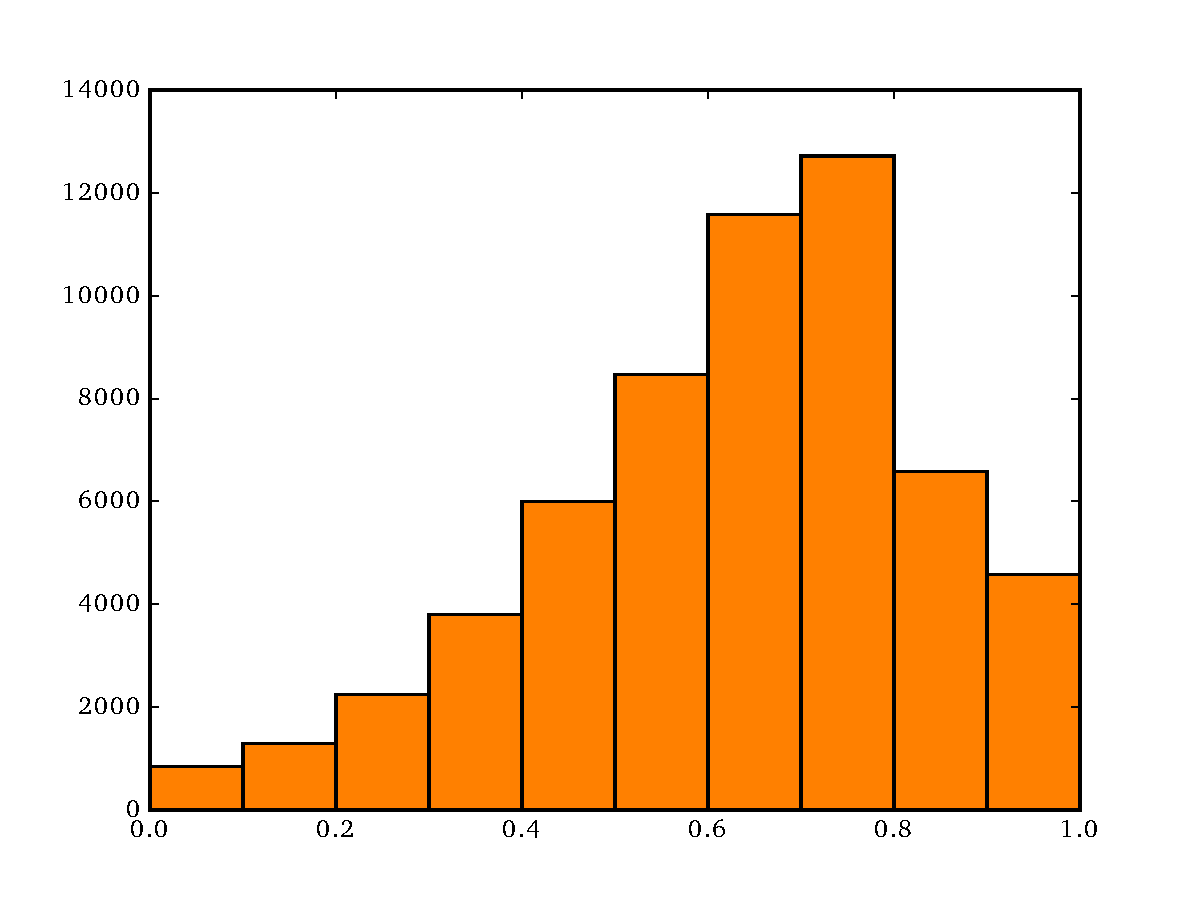
\includegraphics[width=8cm]{cosine_same.pdf}
      \caption{%
        \begin{varwidth}[t]{10cm}
        Repartition of the cosine similarity between \\
        deep vectors from the same speaker
        \end{varwidth}}
      \label{cos_same}
  \end{figure}
\end{frame}

\begin{frame}
  \frametitle{Repartition histograms}
  \begin{figure}[!h]
      \centering
      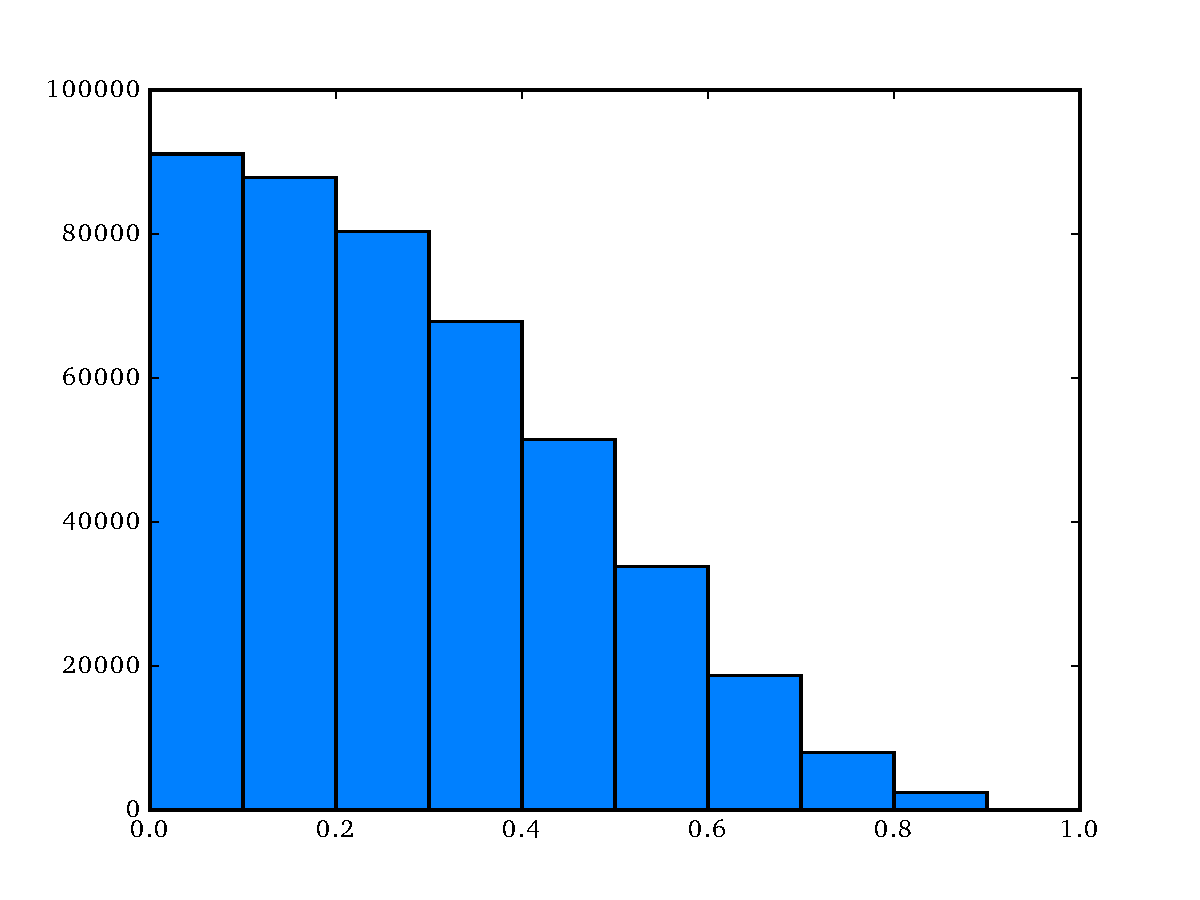
\includegraphics[width=8cm]{cosine_diff.pdf}
      \caption{%
        \begin{varwidth}[t]{10cm}
        Repartition of the cosine similarity between \\
        deep vectors from different speakers
        \end{varwidth}}
  	\label{cos_diff}
  \end{figure}
\end{frame}

\begin{frame}
  \frametitle{Repartition histograms}
  \begin{figure}[!h]
      \centering
      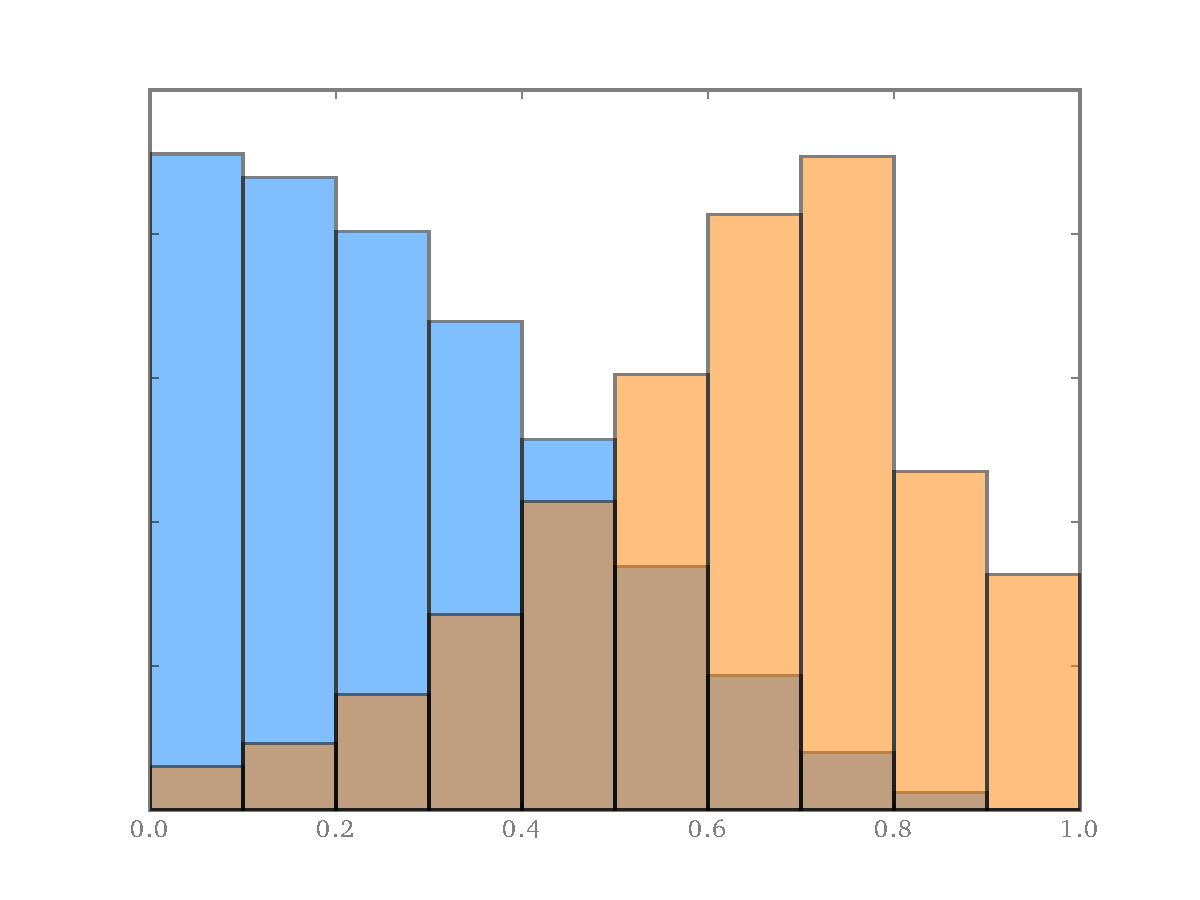
\includegraphics[width=8cm]{cosine_both.pdf}
      \caption{%
        \begin{varwidth}[t]{10cm}
        Repartition of the cosine similarity between deep vectors\\

        \end{varwidth}}

  	\label{cos_diff}
  \end{figure}
\end{frame}


\begin{frame}
  \frametitle{t-Distributed Stochastic Neighbor Embedding (t-SNE)}
  \begin{figure}[!h]
      \centering
      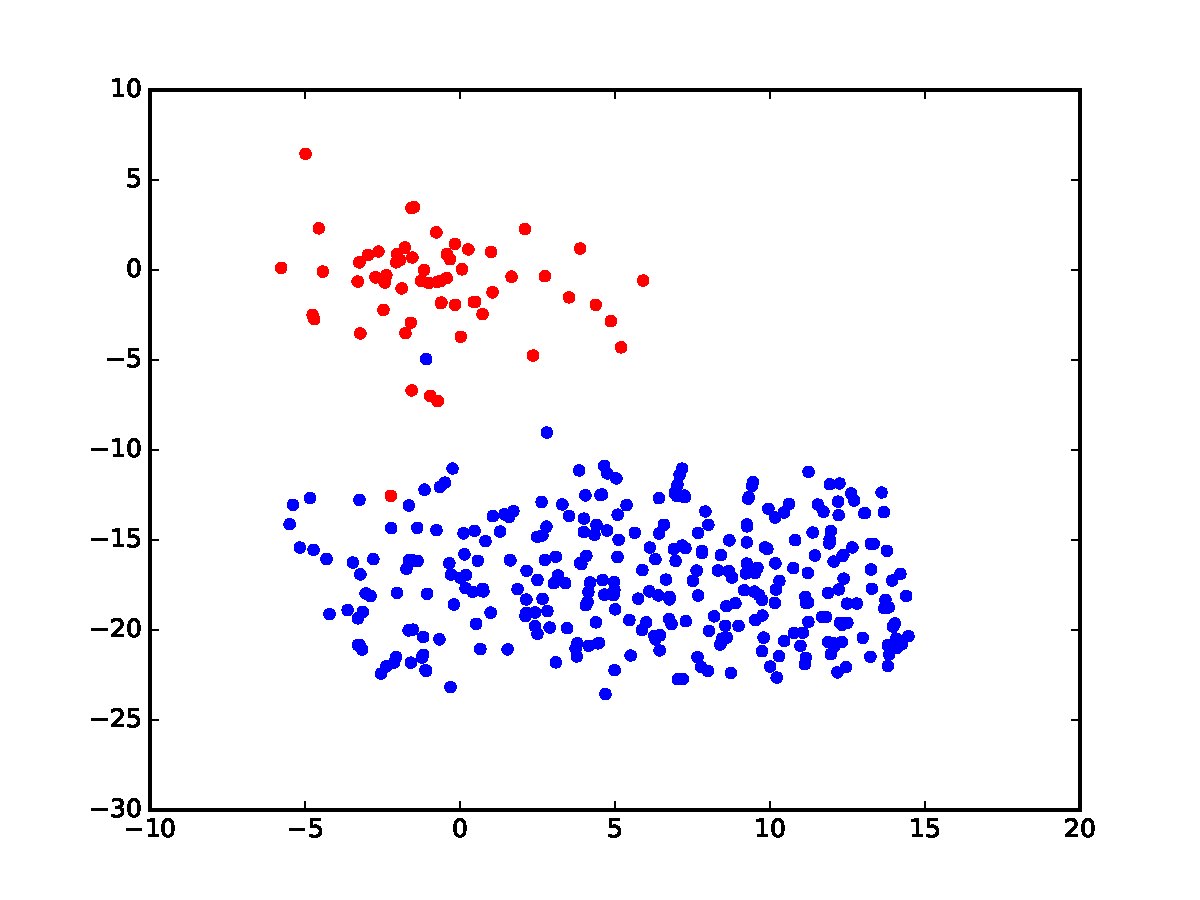
\includegraphics[width=8cm]{../secondNet/tSNE_HOUDIN_TRUCHOT.pdf}
      \caption{t-SNE of the deep vectors of two different speakers}
  \end{figure}
\end{frame}


\begin{frame}
  \frametitle{Detection Error Tradeoff (DET) graph}
  \begin{figure}[!h]
      \centering
      \only<1>{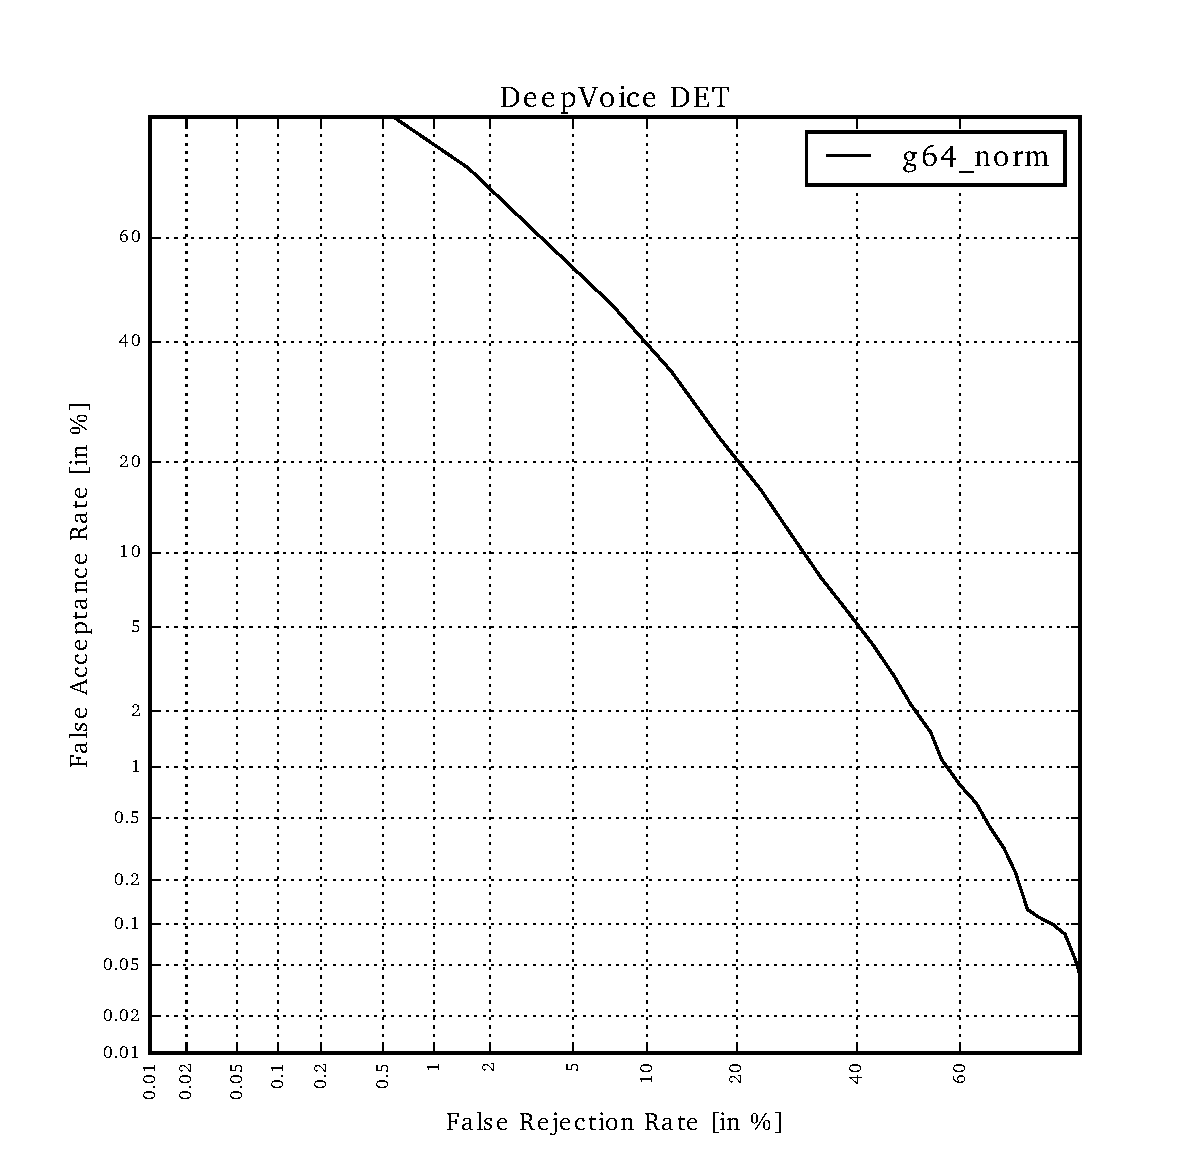
\includegraphics[width=7.5cm]{../scores/det_.pdf}}
      \only<2>{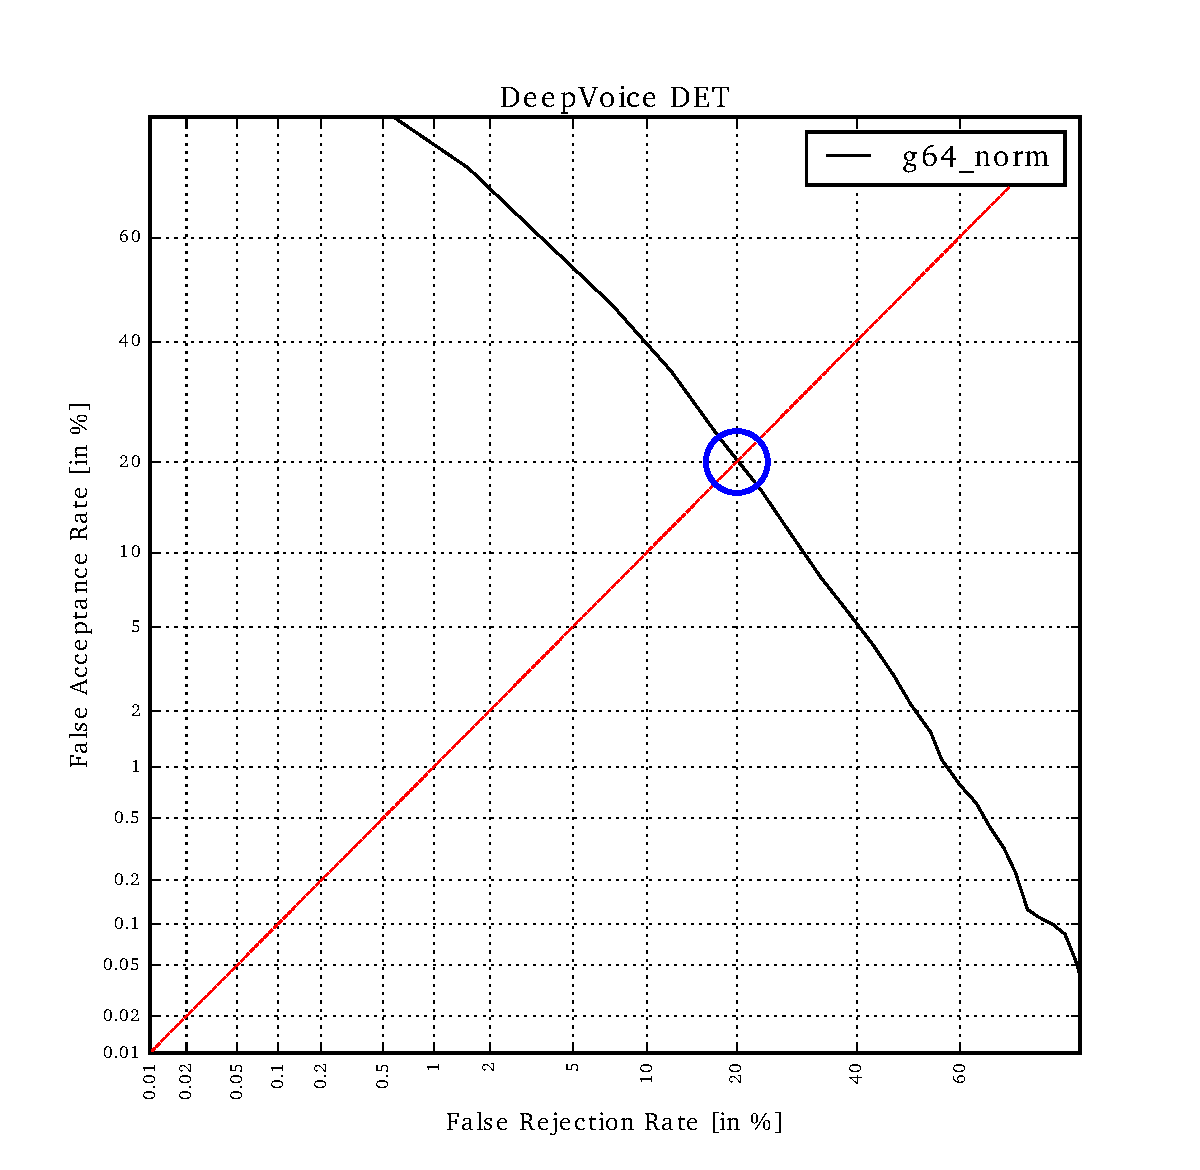
\includegraphics[width=7.5cm]{../scores/det__.pdf}}
  \end{figure}
\end{frame}


\newcommand\experiment[6]{%
  \begin{frame}
    \frametitle{Experiment #1}
    \begin{columns}
      \only<1>{\column{0.6\textwidth}}
      \only<2>{\column{0.35\textwidth}}
        \begin{table}
          \centering
          \resizebox{\columnwidth}{!}{%
          \begin{tabular}{|c|c|c|c|c|c|c|c|}
            \hline
            Number of layers & \multicolumn{#2}{c|}{#2} \\ \hline
            Size of layers   & #3                       \\ \hline
            Tied weights     & \multicolumn{#2}{c|}{#4} \\ \hline
            Optimizer        & \multicolumn{#2}{c|}{#5} \\ \hline
            Dropout          & \multicolumn{#2}{c|}{#6} \\ \hline
          \end{tabular}
          }
        \end{table}
      \only<1>{\column{0.35\textwidth}}
      \only<2>{\column{0.6\textwidth}}
      \begin{figure}[!h]
          \centering
          \includegraphics[width=\columnwidth]{../scores/det#1.pdf}
      \end{figure}
    \end{columns}
  \end{frame}
}



\experiment{0}{5}{2304 & 1000 & 50 & 10000 & 2304}{No}{Gradient Descent}{0.90}
\experiment{1}{5}{2304 & 1000 & 50 & 10000 & 2304}{No}{Adam}{0.90}
\experiment{2}{5}{2304 & 480 & 100 & 480 & 2304}{No}{Adam}{0.90}
\experiment{3}{7}{2304 & 720 & 225 & 70 & 225 & 720 & 2304}{No}{Adam}{0.90}
\experiment{4}{7}{2304 & 720 & 225 & 70 & 225 & 720 & 2304}{Yes}{Adam}{0.90}
\experiment{7}{5}{2304 & 500 & 80 & 500 & 2304}{No}{Adam}{0.80}


\section{Conclusion}

\begin{frame}
  \frametitle{Deep-vectors vs. i-vectors}
  \begin{figure}[!h]
      \centering
      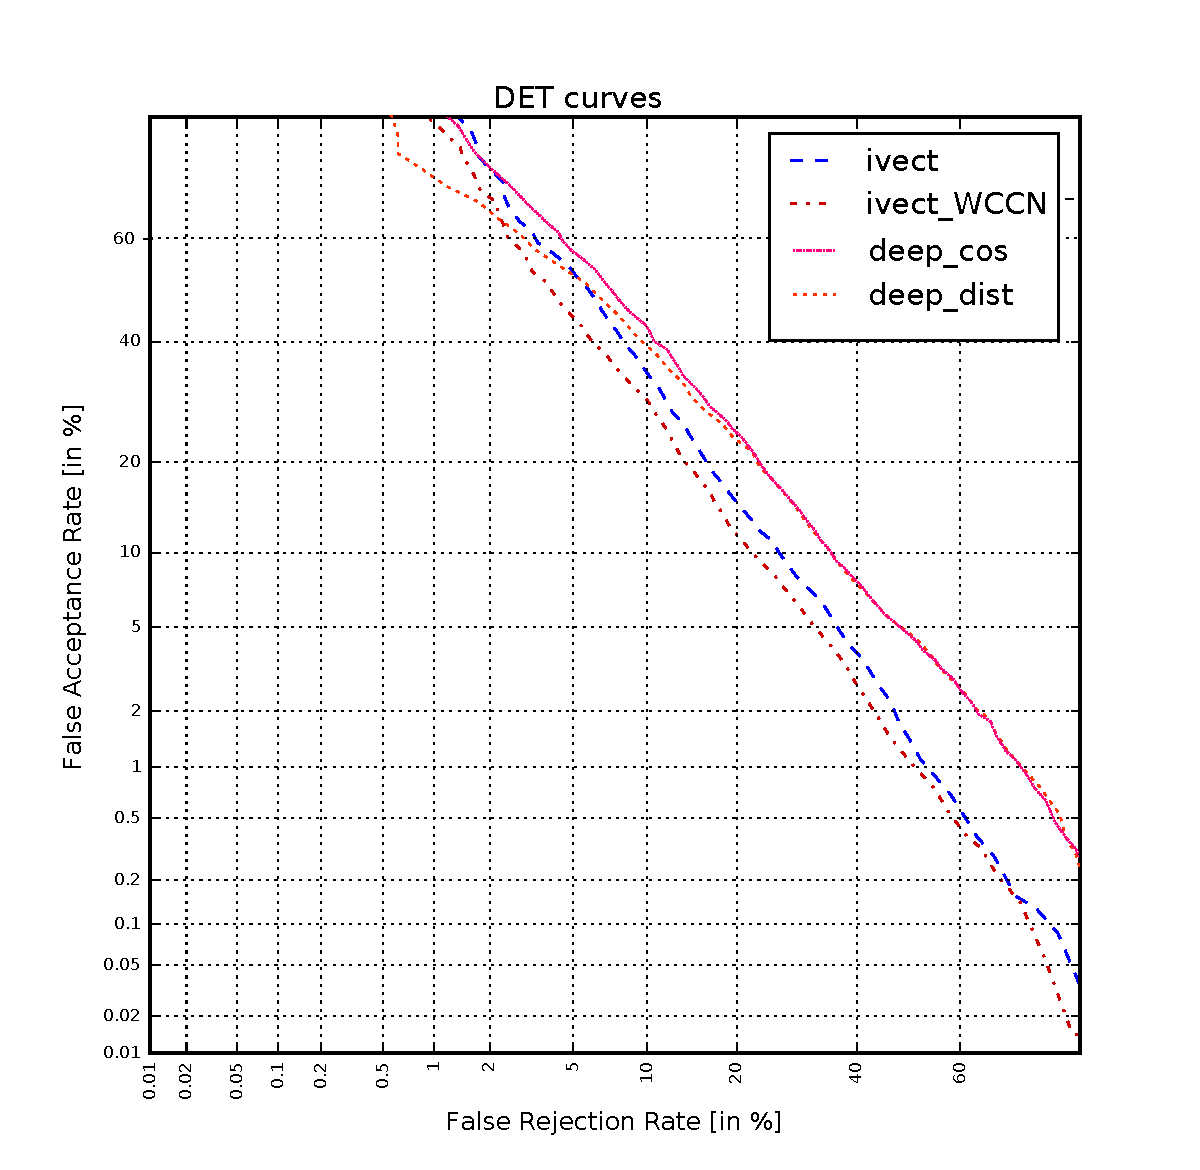
\includegraphics[width=7cm]{../scores/exp7_et_gabi.pdf}
  \end{figure}
\end{frame}


\begin{frame}
  \frametitle{Further work}
  \begin{itemize}
    \item Run additional experiments
    \item Adjust the hyper-parameters
    \item Run more experiments with disjoint training set and evaluation set
  \end{itemize}
\end{frame}

\end{document}
